\documentclass{sigchi}

% Use this command to override the default ACM copyright statement (e.g. for preprints). 
% Consult the conference website for the camera-ready copyright statement.


%% EXAMPLE BEGIN -- HOW TO OVERRIDE THE DEFAULT COPYRIGHT STRIP -- (July 22, 2013 - Paul Baumann)
% \toappear{Permission to make digital or hard copies of all or part of this work for personal or classroom use is 	granted without fee provided that copies are not made or distributed for profit or commercial advantage and that copies bear this notice and the full citation on the first page. Copyrights for components of this work owned by others than ACM must be honored. Abstracting with credit is permitted. To copy otherwise, or republish, to post on servers or to redistribute to lists, requires prior specific permission and/or a fee. Request permissions from permissions@acm.org. \\
% {\emph{CHI'14}}, April 26--May 1, 2014, Toronto, Canada. \\
% Copyright \copyright~2014 ACM ISBN/14/04...\$15.00. \\
% DOI string from ACM form confirmation}
%% EXAMPLE END -- HOW TO OVERRIDE THE DEFAULT COPYRIGHT STRIP -- (July 22, 2013 - Paul Baumann)


% Arabic page numbers for submission. 
% Remove this line to eliminate page numbers for the camera ready copy
\pagenumbering{arabic}


% Load basic packages
\usepackage{balance}  % to better equalize the last page
\usepackage{graphics} % for EPS, load graphicx instead
\usepackage{times}    % comment if you want LaTeX's default font
\usepackage{url}      % llt: nicely formatted URLs

% llt: Define a global style for URLs, rather that the default one
\makeatletter
\def\url@leostyle{%
  \@ifundefined{selectfont}{\def\UrlFont{\sf}}{\def\UrlFont{\small\bf\ttfamily}}}
\makeatother
\urlstyle{leo}


% To make various LaTeX processors do the right thing with page size.
\def\pprw{8.5in}
\def\pprh{11in}
\special{papersize=\pprw,\pprh}
\setlength{\paperwidth}{\pprw}
\setlength{\paperheight}{\pprh}
\setlength{\pdfpagewidth}{\pprw}
\setlength{\pdfpageheight}{\pprh}

% Make sure hyperref comes last of your loaded packages, 
% to give it a fighting chance of not being over-written, 
% since its job is to redefine many LaTeX commands.
\usepackage[pdftex]{hyperref}
\hypersetup{
pdftitle={SIGCHI Conference Proceedings Format},
pdfauthor={LaTeX},
pdfkeywords={SIGCHI, proceedings, archival format},
bookmarksnumbered,
pdfstartview={FitH},
colorlinks,
citecolor=black,
filecolor=black,
linkcolor=black,
urlcolor=black,
breaklinks=true,
}

% create a shortcut to typeset table headings
\newcommand\tabhead[1]{\small\textbf{#1}}


% End of preamble. Here it comes the document.
\begin{document}

\title{Play With Glasses : Exploring Game Design Space On Google Glass}

\numberofauthors{3}
\author{
  \alignauthor 1st Author Name\\
    \affaddr{Affiliation}\\
    \affaddr{Address}\\
    \email{e-mail address}\\
    \affaddr{Optional phone number}
  \alignauthor 2nd Author Name\\
    \affaddr{Affiliation}\\
    \affaddr{Address}\\
    \email{e-mail address}\\
    \affaddr{Optional phone number}    
  \alignauthor 3rd Author Name\\
    \affaddr{Affiliation}\\
    \affaddr{Address}\\
    \email{e-mail address}\\
    \affaddr{Optional phone number}
}

\maketitle

\begin{abstract}
hi I'm abstract
\end{abstract}

% \keywords{
% 	Guides; instructions; author's kit; conference publications;
% 	keywords should be separated by a semi-colon.
% 	\textcolor{red}{Mandatory section to be included in your final version.}
% }

% \category{H.5.m.}{Information Interfaces and Presentation (e.g. HCI)}{Miscellaneous}

% See: \url{http://www.acm.org/about/class/1998/}
% for more information and the full list of ACM classifiers
% and descriptors. 
% \textcolor{red}{Mandatory section to be included in your
% final version. On the submission page only the classifiers'
% letter-number combination will need to be entered.}


\section{Introduction}

% \begin{itemize}
% \item wearable device 是趨勢拉!!
% \item google glass 是最有希望的Wearable device拉!!
% \item 傳統行動裝置的應用程式有80\%是遊戲啦!!所以google Glass上的遊戲很有商業潛力啦!!
% \item Google Glass上的遊戲設計是一個unexplored area啦!!
% \item 我們run 了一個24人的user study 發現相較于傳統的Game Design Guideline,Google Glass上的遊戲有三個不同Topic,分別是Control,Eye Tiring,Social Acceptable.


% \item 我們根據user imagination的統計, 我們選擇製作了一個完整的第一人稱射擊遊戲來Explore Glass Game 的Design Space。
% \item 我們分別Run了User Study 2,User Study 3, User Study 4來更加深入的探討Control,Eye Tiring,Soical三個Topic。
% \end{itemize}

% One of the major recent wearable computing breakthroughs is Google’s new ‘eyewear computer’, expected to be commercially available in 2014, referred to as Glass ~\cite{googleglass}. Eyewear computers are claimed to be the next evolution beyond smartphones.
 
% Recent statistics show that around 70-80\% of all mobile downloads is composed of mobile games~\cite{statistics,infographic}. Such a large craze for ludic engagements in mobile environment has made it an industry of high scope and visibility. As such, survey reports predict a rise of up to \$54 billion in revenue by 2015 ~\cite{statistics,infographic}.

\begin{enumerate}
\item Without a doubt ``Wearable Device'' is the trend of the future!!!!!
\item It's true that ``Google Glass'' is the most hopeful device!!!!!
\item 80\% of the App are ``Game'' in traditional mobile device!!!!! So we can make sure that Google Glass has deeply commercial prospection.
\item Game Design on Google Glass is an unexplored area so far.
\item We had already run 24 person for user study. Compared to traditional game design guideline, games on google glass can divide in three different topic, ``Control'', ``Eye tiring'', ``Social acceptable'' respectively.
\item From the statistics of our user imagination, we decide to produce a complete first-person shooter(FPS) game to explore the design space on glass game.
\item Afterwards, we will run user study 2, user study 3, and user study 4 to deeply analyze and discuess our three main topic(Control, Eye tiring, and Social acceptable).
\end{enumerate}

One of the major recent wearable computing breakthroughs is Google’s new ‘eyewear computer’, expected to be commercially available in 2014, referred to as Glass ~\cite{googleglass}. Eyewear computers are claimed to be the next evolution beyond smartphones.
 
Recent statistics show that around 70-80\% of all mobile downloads is composed of mobile games~\cite{statistics,infographic}. Such a large craze for ludic engagements in mobile environment has made it an industry of high scope and visibility. As such, survey reports predict a rise of up to \$54 billion in revenue by 2015 ~\cite{statistics,infographic}.


\section{Related Work}

Although there is lack of offcial research focusing on glass game design, we still can borrow some experience from the research on existing game design and head-mounted device control.


\subsection{Game Design}

There are tons of research focusing on design guideline or heuristic rule for traditional video games\cite{gameflow,criticalreview,chi04game,09game,02game,08game,07game}. Nevertheless, after the smart phone hitting the market, game design for mobile phones also became a hot research topic\cite{mobilegame,mobile06,mobile08,icec06}. Besides video and mobile game, there are only bits and pieces research on other specific platform. For example, Elena et al. focused on using their unique gaming hardware, ``Body Bug'', to explore body games\cite{bodygame}; Wetzel et al. explored the game design in augmented reaility\cite{argame}; Mueller et al. presented a set of guidelines for movement-based game design\cite{movegame}. Bertelsmeyer et al. provided an innovative wearable game and researched in how to consider the characteristics of today's wearable hardware when developing a game\cite{wearable}. Unfortunately, they didn't consider the smart glass as a gaming platform in their research. 

From the previous research on related field, although there are no research focusing on glass game design, some previous game design guidelines are platform independent and we can use it directly. For instance, Pinelle et al.\cite{videogame} developed game heuristics in 10 categories, most of them are platform independent. 
Such as ``Predictability'' issue , games should respond to users' actions in a predictable manner. And ``Game status'' issue, game UI does provide adequate information on character, game world, or enemies, visual indicators, icons, and maps. 

In this paper, we focus on glass game design, and we only explore new issues which do not exist in traditional game design.


\subsection{Head Gesture-based Control}

Head gesture-based controls was explored by some previous works. LoPresti et al.\cite{neck} studied the human ability to use head gesture-based control. They modeled the relationship between neck functional range and accuracy/speed in icon selection; Hinkel et al.\cite{wheel} designed a system that allowed individuals to control a motorized wheelchair with simple head movements; Malkewitz et al.\cite{headdesktop} tried to map mouse and keyboard to speech and head motion, and enabled the possibility to add alternative input channels to common personal computers at moderate costs; Crossan et al.\cite{tilt} explored head tilting as an input technique to allow a user to interact with a mobile device ``hands free''; Zhu et al.\cite{tele} compared three different cameras' viewpoint control models and indicated the advantages of using the natural interaction model(combining eye gaze and head motion); Joseph et al.\cite{robot} explored the capabilities of head tracking combining with head mounted displays(HMD) as an input modality for robot navigation; Greuter et al.\cite{viewport} presented the use of commodity depth based cameras to control viewpoint from passive unencumbered head tracking. This allowed participants to maintain correct perspective while playing an immersive computer ball game.

Base on previous work, we can realize that head gesture-based control are really powerful for application. By using google glass, we can sense head gesture directly by glass gyro. However, how to use head gesture in glass game design is still an open question. In this work, we let users try different control style and explore the rule of using head gesture in glass game.




\section{User Study 1}

% \begin{enumerate}
% \item Process of gameplay
% \item User's feedback for existing games
% \item User's imagination
% \end{enumerate}

In order to realize the current game play experience on google glass. We use games currently existing on google glass to perform our user study. Furthermore, with a view to understanding the response and feedback for different control style and game content from users, we choose four games, ``Balance'', ``Shape Splitter'', ``Matcher'', and ``Clay Shooter'', with unique control type respectively(see Table~\ref{tab:gameControlTypes}).


About our process, we gave user five minutes to play each game, and filled in a questionnaire to understand the positive and negitive feedback from users after playing each game. To make results effective, the order of the game were counterbalanced to eliminate the effects of ordering. After playing all four games, we also provided a final questionnaire to realize the whole glass game play experience from users.


We recruit 24 users (16 males,8 females) with average 23.8 years old (std 3.96) and 13.9 years game experience(std 5.96). To avoid bias cause by myopia, which might affect game expereience if you are not playing google glass with your own shortsight degree lens, we only recruit the user who don't have myopia or wearing contact lens. All of our user has no experience wearing google glass before.



\begin{table}[!h]
\newcommand{\tabincell}[2]{\begin{tabular}{@{}#1@{}}#2\end{tabular}}
   \centering
   \begin{tabular}{|p{0.4\columnwidth}|p{0.4\columnwidth}|}
     \hline
     % \tabhead{Objects} &
     \multicolumn{1}{|p{0.3\columnwidth}|}{\centering\tabhead{Game}} &
     \multicolumn{1}{|p{0.5\columnwidth}|}{\centering\tabhead{Control}} \\
     \hline
     Balance & gyro\\
     \hline
     Shape Splitter & in-air gesture\\
     \hline
     Matcher & gyro, tap\\
     \hline
     Clay Shooter & gyro, voice control\\
     \hline
   \end{tabular}
   \caption{Game control types}
   \label{tab:gameControlTypes}
 \end{table}



\subsection{User feedback}
We collect totally 304 feedback from users (141 positive feedback,163 negative feedback), after reviewing all feedback, we found that some feedback is not glass related. For instance ,user might complain about the level design or visual art and admire to the innovative game design or good to listen music.

Focusing on Glass too long is not comfortable
Gyro is comfortable for 1D and 2D control
Gyro with 360 degree is BAD
Voice Control \& In-Air Gesture are NOT social acceptable
tapping is acceptable many tappings are annoying
In air gesture is tiring
Current in air gesture detecting sucks
Voice control always out of control



\begin{table}[!h]
\newcommand{\tabincell}[2]{\begin{tabular}{@{}#1@{}}#2\end{tabular}}
   \centering
   \begin{tabular}{|p{0.4\columnwidth}|p{0.3\columnwidth}|}
     \hline
     % \tabhead{Objects} &
     \multicolumn{1}{|p{0.3\columnwidth}|}{\centering\tabhead{Category}} &
     \multicolumn{1}{|p{0.5\columnwidth}|}{\centering\tabhead{User Feedback}} \\
     \hline
     Focusing on Glass too long is not comfortable & \tabincell{c}{p1: hihi I'm p1. I'm feedback.\\p2: hihi I'm p2. I'm feedback2.} \\
     \hline
     Gyro is comfortable for 1D and 2D control & \\
     \hline
     Gyro with 360 degree is BAD & \\
     \hline
     Voice Control \& In-Air Gesture are NOT social acceptable & \\
     \hline
     tapping is acceptable many tappings are annoying & \\
     \hline
     In air gesture is tiring & \\
     \hline
     Current in air gesture detecting sucks & \\
     \hline
     Voice control always out of control & \\
     \hline
   \end{tabular}
   \caption{Small Sun.}
   \label{tab:table1}
 \end{table}

 \begin{table}[!h]
\newcommand{\tabincell}[2]{\begin{tabular}{@{}#1@{}}#2\end{tabular}}
   \centering
   \begin{tabular}{|p{0.4\columnwidth}|p{0.3\columnwidth}|}
     \hline
     % \tabhead{Objects} &
     \multicolumn{1}{|p{0.3\columnwidth}|}{Game Play Feedback} &
     \multicolumn{1}{|p{0.5\columnwidth}|}{Level design, Music, Visual art, Casual, Challenge, Game for purpose, Innovative, Physics, Immersion} \\
     % \multicolumn{1}{|p{0.3\columnwidth}|}{\centering\tabhead{Game Play Feedback}} &
     % \multicolumn{1}{|p{0.5\columnwidth}|}{\centering\tabhead{User Feedback}} \\
     \hline
     \multicolumn{1}{|p{0.3\columnwidth}|}{Glass Related Feedback} & 
     \multicolumn{1}{|p{0.5\columnwidth}|}{Gyro, In-air gesture, Tap, Voice control, Eye tiring, Social acceptable, AR} \\
     \hline
   \end{tabular}
   \caption{We collect 304 feedbacks and manually divide into 16 categories.}
   \label{tab:table1}
 \end{table}

% \begin{table}
% \newcommand{\tabincell}[2]{\begin{tabular}{@{}#1@{}}#2\end{tabular}}
%   \centering
%   \begin{tabular}{|c|c|c|}\hline
% 1 & \tabincell{c}{the first line \\ the next\\the next\\ last} & \tabincell{c}{one \\ one}\\\hline
% 2 & \tabincell{c}{hello\\ aha\\ ok \\yes \\en} & \tabincell{c}{two \\ two \\ two} \\\hline
% \end{tabular}
%   \caption{longtitle}
% \end{table}

\begin{figure}[!t]
\centering
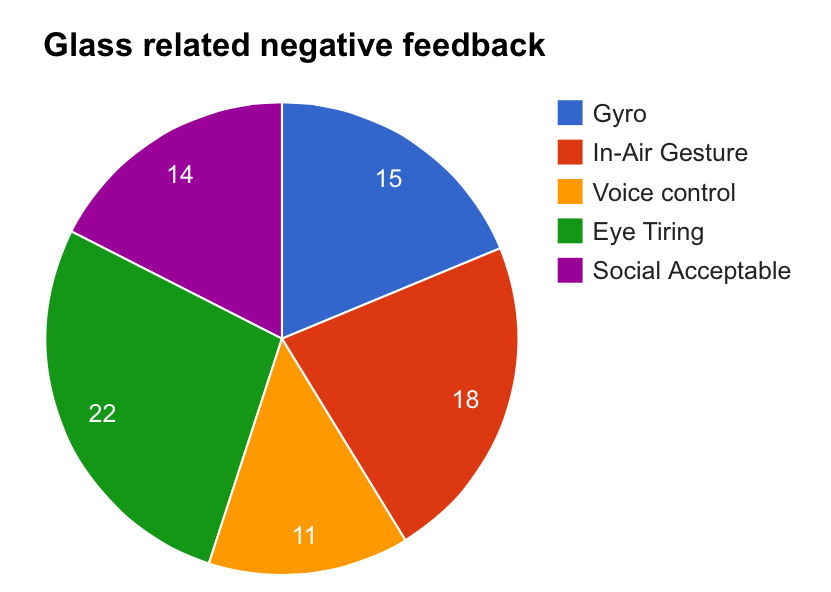
\includegraphics[width=0.9\columnwidth]{Figures/US1_userfeedbackStatistics.png}
\caption{Hi I'm Small Sun.}
\label{fig:PS_Frus}
\end{figure}


\subsection{Observation}
% \begin{enumerate}
% \item NOT social acceptable != NOT fun
% \item Small movement is better
% \end{enumerate}
From user feedback, although social acceptable would make an influence on glass game play experience, most users still think game play experience is fun and interesting. With this condition, we can conclude that social acceptable is independent to the level of fun and enjoyment. In other words, if a game has low social acceptable rate, it does not mean the game is not fun or users don't like it. In addition, we also find that small movement interacting with google glass is better and more perferred for users. 


\subsection{User imagination}
After playing all four games, we also asked users to imagine what kind of games on google glass will they like the most in user study 1. With existing glass game scene and users' originality, they brought up thirty-seven interesting glass game scenario in total. We divided them into six types of game, ``First-Person Shooter'', ``Reality Puzzle Game'', ``Social Game'', ``Sport Game'', ``Management Game'', and ``Others'' respectively (see Figure~\ref{fig:US1_TypesOfGame}). We also found that one-third of users want like first-person shooter game the most. So we decided to implement a first-person shooter game which will support multiple types of control style for users. With this design, not only users can choose which control type they like the most by their own, but we also can find out the best control style from users' feedback for first-person game on google glass and design a guideline to make better game play experience.

\begin{figure}[!t]
\centering
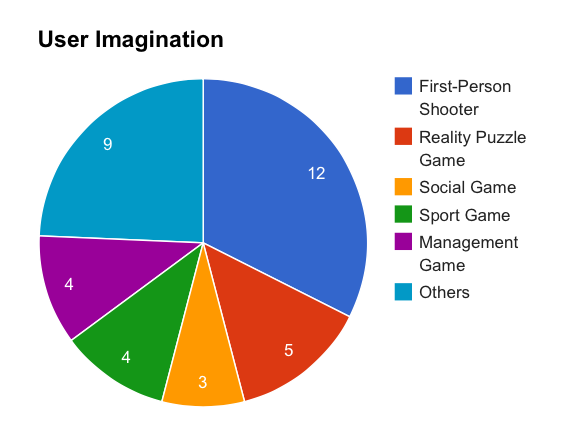
\includegraphics[width=0.9\columnwidth]{Figures/US1_userImaginationStatistics.png}
\caption{Hi I'm Small Sun 2.}
\label{fig:US1_TypesOfGame}
\end{figure}

\section{Game Prototype}

To get deeper understanding of glass game design, we have to build a game by ourself, so that we can have some control variable to do direct compare with different settings. According to the user imagination from user study 1, there are five different game type player suggested. We choose FPS as our game type, because there are most user want to play FPS game, and there are most control issues in this game type. We expect we can satisfy most user and get most useful knowledge by studying and implement this game type.



\subsection{Control}
There are 4 main controls in FPS game, the first one is the viewport control, it's about how user to change camera perspection and observe the surrounding environment. The second one is aim control, how does player to aim their enemy target. The third one is fire control, how does player trigger the fire to beat the enemy. The fourth is the move control, how does player to control avator position and dodge the bullet from enemy.

Smart Glass are not meant to replace smart phone\cite{lecture}, they should complement the insufficient of each other. And google glass are designed to be always connect with smart phone through bluetooth. So we include smart phone as controller as a candidate in design of our control scheme.

According to previous work\cite{headvideo,tele,robot,viewport}, using head orientation as viewport control is no doubtly intuitive and user prefered because of the metaphor of moving our own head. But is using head orientation really suitable for users to aim the target is not confirmed. So we supposed 3 different aim control schemes to confirm which would be the user's favorite. The 3 different aim control schemes is listing here:

\begin{enumerate}
\item Viewport aiming scheme : The most traditional one method, just put a sight bead in the center of viewport, player can aim the enemy by moving their view port. In another word, player are using head orientation to aim the target.

\item Gun aiming scheme : Consider you smart phone as a small gun and use your phone orientation to aim the target. The sight bead will show on the google glass screen to help user do micro movement aiming.

\item Phone joystick scheme : Using smart phone as a joystick to move the sight bead on the glass screen.
\end{enumerate}

We supposed 3 different firing controls as below :
\begin{enumerate}
\item Phone trigger scheme : Use the touch screen on mobile phone as the firing trigger, player just fire by tapping on their phone.

\item Glass tapping scheme : Player use finger to tap on glass touch pad to trigger gun fire.

\item Voice control scheme : Player use voice control like the sound of ``Bang'' to tirgger gun fire.

\item Blink eye scheme : Player use intentional eye blinking as a fire trigger.
\end{enumerate}

We supposed 3 moving control scheme :

\begin{enumerate}
\item Head gesture scheme : We borrow the control style from the work of Hinkel et al.\cite{wheel}, and implement the system in our FPS game control system.

\item Phone controller scheme : Using smart phone as a joystick to move the player by manipulating the touch screen.

\item On track moving scheme : This is a trick one, we can't exclude the possibility that control player movement is not suitable for glass game. In this scheme we design a pre-defined track for player, and player will move on the track automaticlly. So player can focus on aiming and fighting, then ignore the movement control.
\end{enumerate}

%\subsection{Art Style}

%\subsection{Eye tiring}

%\subsection{Social Acceptable}

\subsection{Implementation}
We use Unity3D \cite{unity} to develop our game. 

%But our user study 1 indicate that force player to rotate their head with too big degree is uncomfortable.
\section{User Study 2}

We want to realize what's a good gyro control. 

\begin{enumerate}
\item Range of gyro movement\\
ask them directly.
\item The precision of gyro(relavent target size?)\\
observe data.
\end{enumerate}

\subsection{Result expectation}

\begin{figure}[!t]
\centering
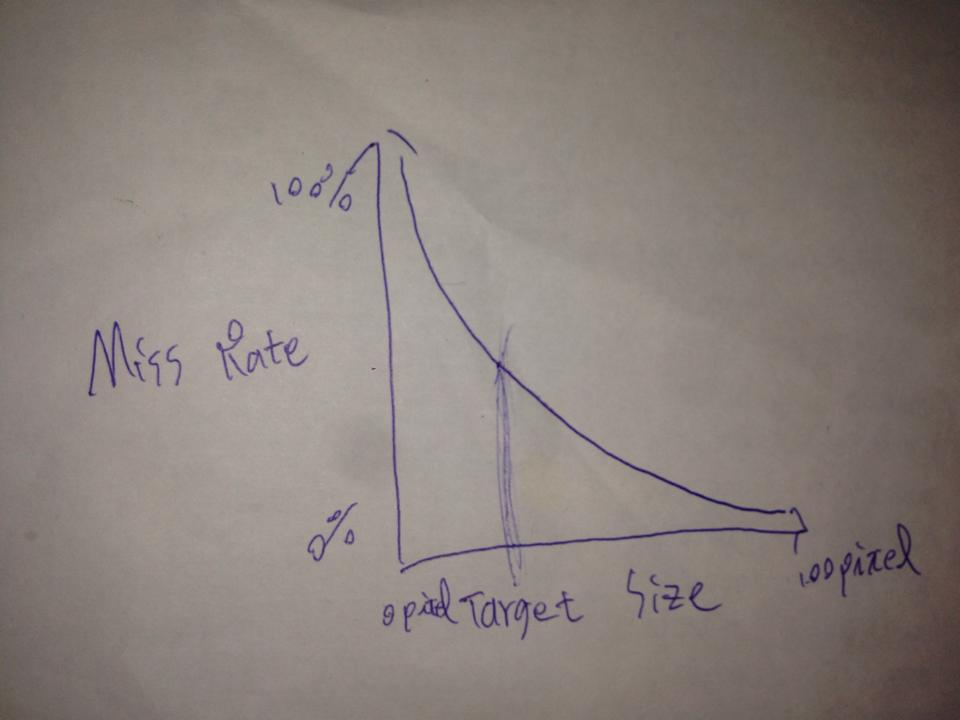
\includegraphics[width=0.9\columnwidth]{Figures/US2_missRate.jpg}
\caption{Hi I'm Small Sun.}
\label{fig:PS_Frus}
\end{figure}

\begin{figure}[!t]
\centering
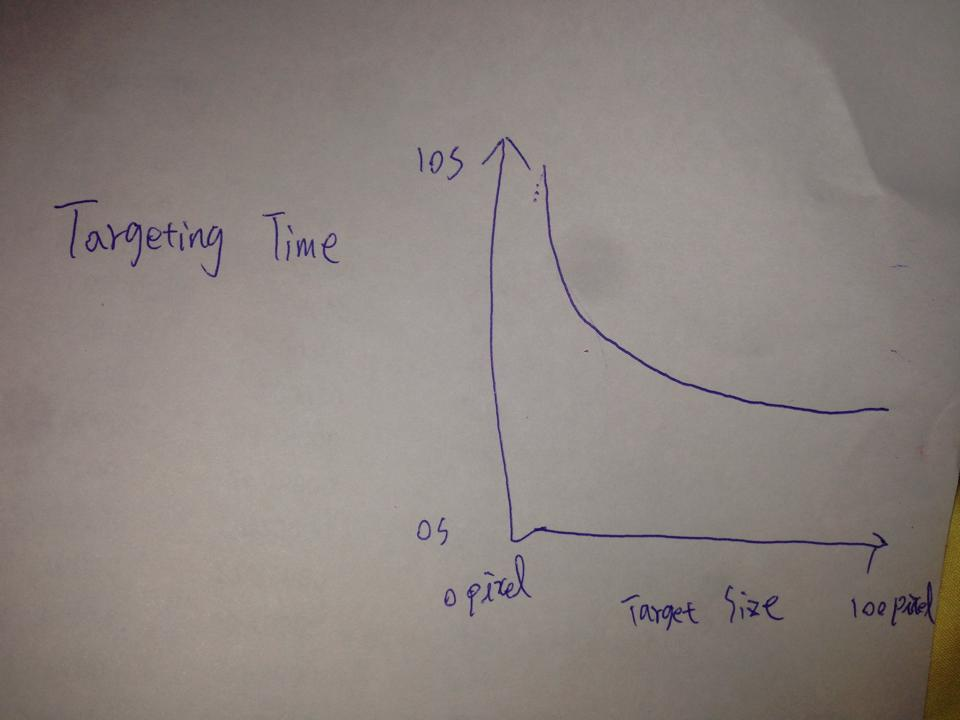
\includegraphics[width=0.9\columnwidth]{Figures/US2_targetingTime.jpg}
\caption{Hi I'm Small Sun.}
\label{fig:PS_Frus}
\end{figure}

\begin{figure}[!t]
\centering
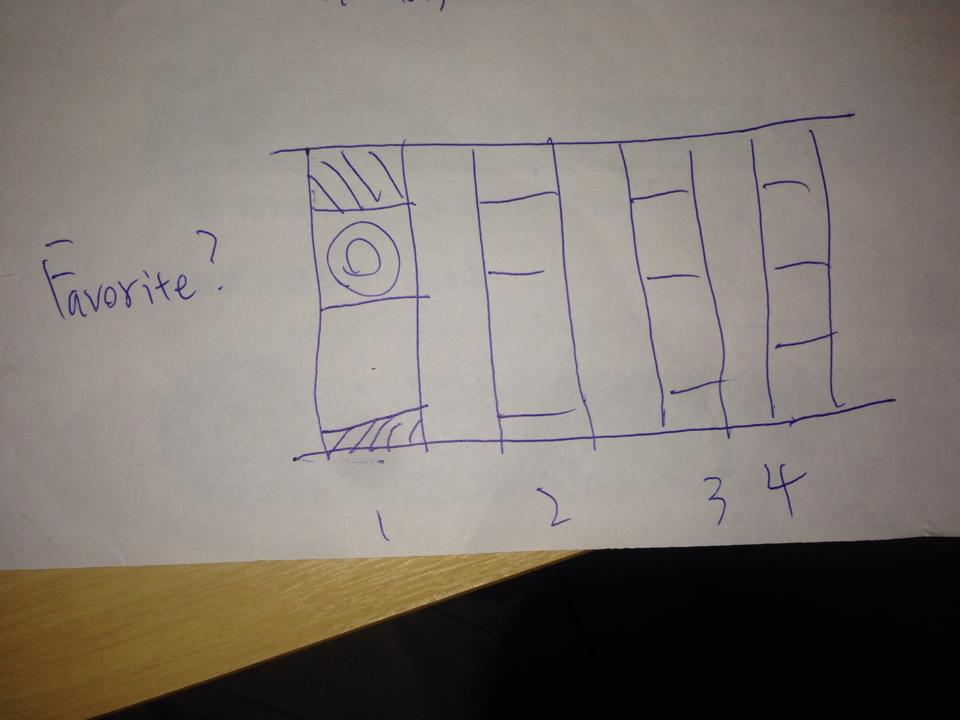
\includegraphics[width=0.9\columnwidth]{Figures/US2_favoriteFire.jpg}
\caption{Hi I'm Small Sun.}
\label{fig:PS_Frus}
\end{figure}

\begin{figure}[!t]
\centering
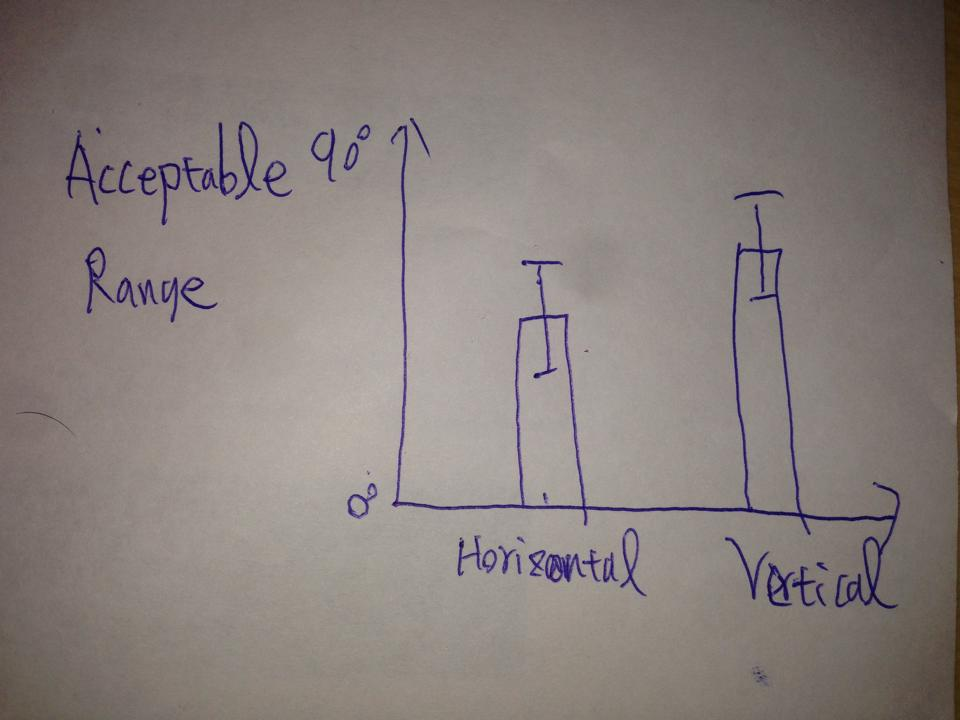
\includegraphics[width=0.9\columnwidth]{Figures/US2_acceptableRange.jpg}
\caption{Hi I'm Small Sun.}
\label{fig:PS_Frus}
\end{figure}

\begin{figure}[!t]
\centering
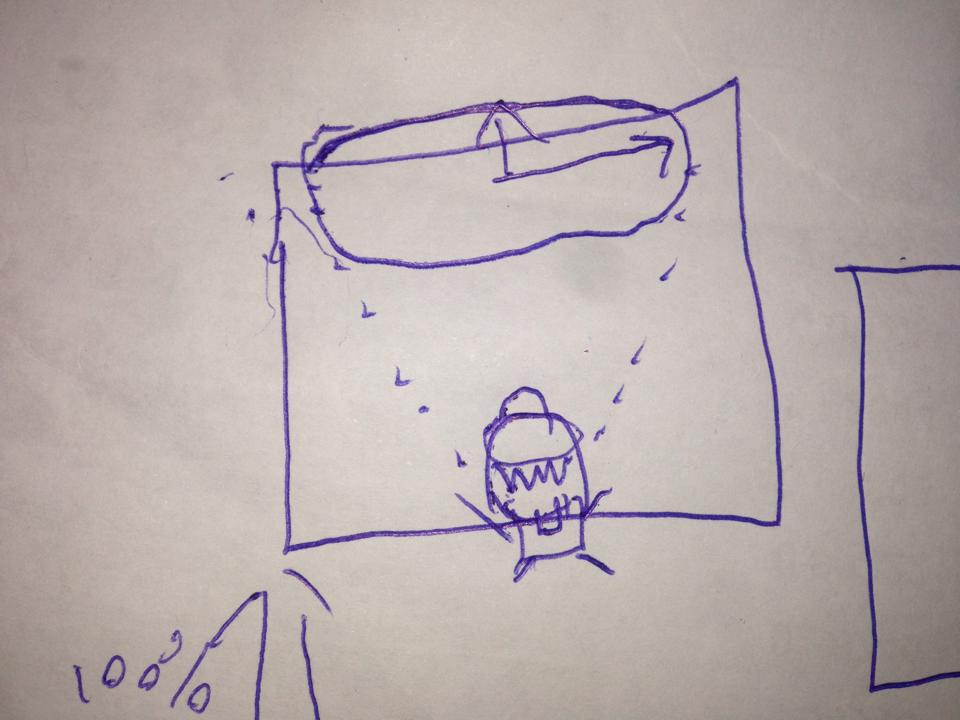
\includegraphics[width=0.9\columnwidth]{Figures/coverPhoto2.jpg}
\caption{Hi I'm Small Sun.}
\label{fig:PS_Frus}
\end{figure}


fire
\begin{enumerate}
\item Use mobile phone
\item Tapping google glass's touch pad
\item Voice control
\item Eye blinking
\end{enumerate}


\section{User Study 3}
goal

We want to realize the relationship between game duration time, eye tiring, and fun of game.

eSFQ...............................?
\begin{enumerate}
\item Time
\item Tiring index 
\item Fun index
\end{enumerate}

\subsection{Result expectation}

\begin{figure}[!t]
\centering
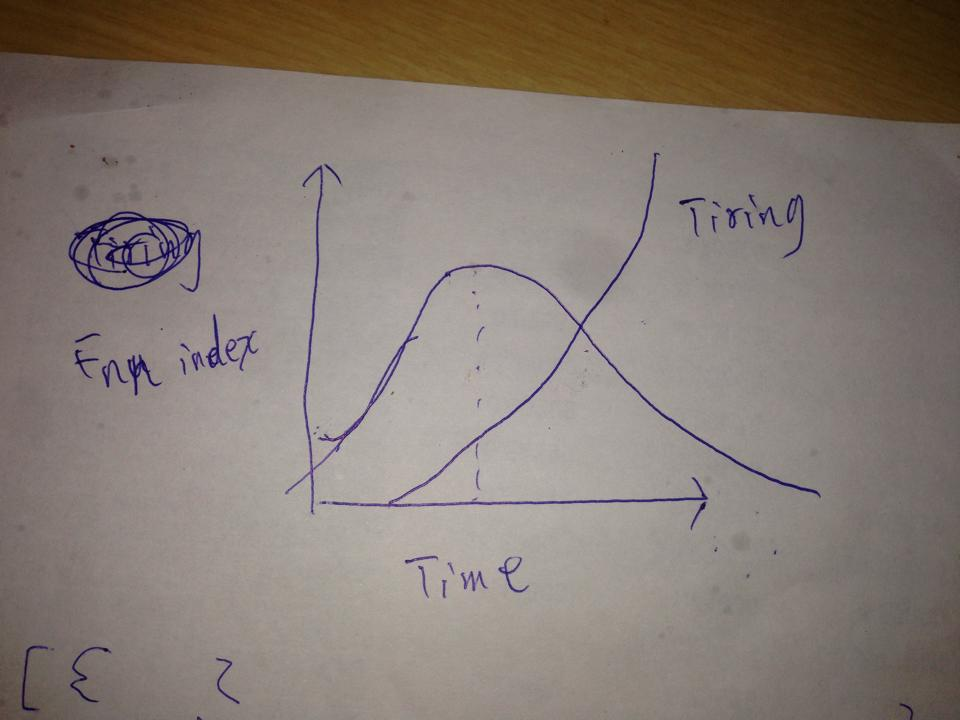
\includegraphics[width=0.9\columnwidth]{Figures/US3_tiringAndFun.jpg}
\caption{Hi I'm Small Sun.}
\label{fig:PS_Frus}
\end{figure}

\section{User Study 4}

We will ask users for favorite fire control.
% The method of fire will be established by the result from user study 2.

The length of game will be set by the result from user study 3.


environment
\begin{enumerate}
\item Private room \\
Single person
\item Restaurant \\
Many people around you but they may focus on their work.
\item On MRT \\
You may be the eye target of everyone around you.
\end{enumerate}

\subsection{Result expectation}

\begin{figure}[!t]
\centering
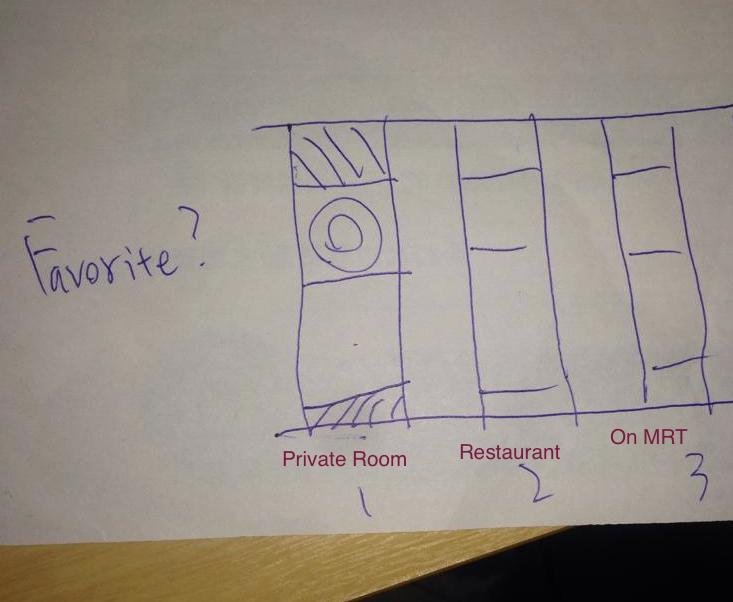
\includegraphics[width=0.9\columnwidth]{Figures/US4_favoriteFire.jpg}
\caption{Hi I'm Small Sun.}
\label{fig:PS_Frus}
\end{figure}

\begin{figure}[!t]
\centering
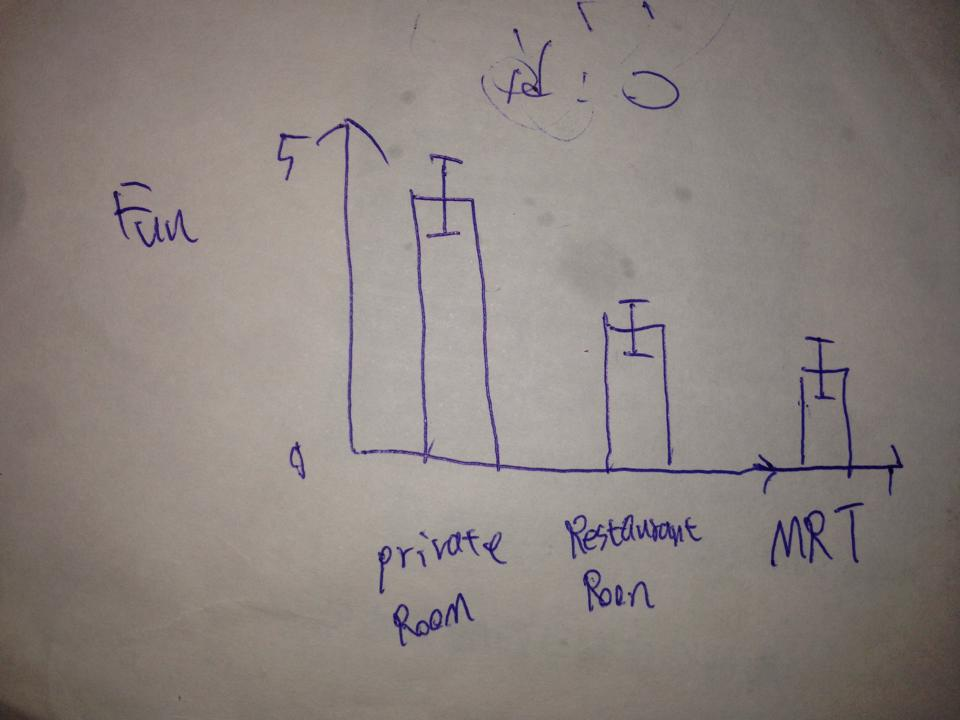
\includegraphics[width=0.9\columnwidth]{Figures/US4_FunAndEnvironment.jpg}
\caption{Hi I'm Small Sun.}
\label{fig:PS_Frus}
\end{figure}



\input{Section/Discussion.tex}
\input{Section/Conclusion.tex}


\balance

\bibliographystyle{acm-sigchi}
\bibliography{sample}
\end{document}
